\chapter{Transversal beam dynamics in circular accelerators} \label{chapter03}

% i build a python tool and explain at each step how i approached the physics

This chapter introduces the important methods and physics of transverse motion of particles in circular accelerators. This thesis only considers the linear order of beam optics, which are called so in analogy to geometrical light optics. Its physical concepts were developed by Courant and Snyder~\cite{courantsnyder}. The following introduction to linear beam optics forms the basis of my python tool.

The books from Klaus Wille~\cite{wille}, Frank Hinterberger~\cite{hinterberger} and Helmut Wiedemann~\cite{wiedemann} are the key sources for this chapter. However the notation and conventions will slightly differ to match the Elegant~\cite{elegant} style, which I used as main reference for my simulations.

\section{Equation of motion of charged particles in magnetic fields}
In this section the equations of motion for linear beam optics are derived. The fundamental force on a particle with the charge $q$ and velocity $v$ is called the \textit{Lorentz force}:
\begin{equation}
	\begin{aligned}[b]
		\textbf{F}_{\textup{L}} = \textbf{F}_\textup{E} + \textbf{F}_\textup{B} = q \: \textbf{E} + q \: \textbf{v} \times \textbf{B}.
	\end{aligned}\label{lorentzforce}
\end{equation}
As an electron in a modern synchrotron radiation source is moving almost with the speed of light~$c_0$ only the magnetic part $\textbf{F}_\textup{B}$ is of particular interest in the following. Electric fields with an effect in the same magnitude are technically not feasible.

The first subsection introduces the standard coordinate system of accelerator physics, which minimizes the mathematical efforts and which is especially helpful for the multipole expansion of the magnetic field in the second subsection. The linear approximation of the equations of motion in the third subsection is the essential foundation for the transfer matrix method in the next section.

\subsection{The co-moving coordinate system}
\begin{figure}
	\centering
	\includegraphics[width = 0.8\textwidth]{images/03-comoving-cartesian-coordinates.pdf}
	\caption{Co-moving curvilinear Frenet-Serret coordinates.}
	\label{fig:comovingcoordinates}
\end{figure}
The ideal beam trajectory in an accelerator is defined by the position and design of its beam guiding magnets. This perfect trajectory is called the \textit{orbit}. It is useful to describe the motion of a particle in relation to it. Therefore we introduce the orthogonal coordinate system $K = (x,y,s)$ whose origin follows along the orbit. This curvilinear coordinate system with the basis vectors
\begin{equation}\begin{aligned}[b]
		 & \uvec{s}(s)= \frac{\du \textbf{r}_0(s)}{\du s} &  & \small\text{unit vector tangent to the orbit} \\
		 & \uvec{x}(s)                                    &  & \small\text{normal (horizontal) unit vector}  \\
		 & \uvec{y}(s)= \uvec{s}(s) \times \uvec{x}(s)    &  & \small\text{binormal (vertical) unit vector}
	\end{aligned}\label{frenetserretvectors}\end{equation}
is also known as \textit{Frenet-Serret system}. While the \textit{s}-axis moves tangential to the orbit, the \textit{x-y} plane is perpendicular to it. The $s$ coordinate is defined by the distance covered on the orbit. The $z$ coordinate corresponds to the path length of the individual particle trajectory. The horizontal and vertical coordinates are labeled with $x$ and $y$. For statements which are valid for both transversal planes we will use the general variable $u$. The horizontal and vertical radii of curvature of the orbit are identified with $\rho_\text{0x}$ and $\rho_\text{0y}$\footnote{In our definition of the Frenet-Serret system the \textit{x}-axis points to the left of the beam direction. Therefore the horizontal and vertical radius of curvature for a particle bended to the right in the direction of travel is positive and vice versa. It is also common to define the \textit{x}-axis so that it points to the right. In such a coordinate system the sign of the curvature would change.}. Accordingly $\kap = \rho_\text{0x}^{-1}$ and $\kapy = \rho_\text{0y}^{-1}$ are the horizontal and vertical curvatures of the orbit, respectively.
\begin{figure}
	\centering
	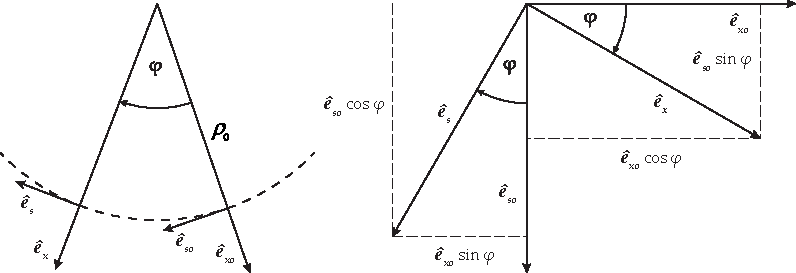
\includegraphics[width = 0.95\textwidth]{images/03-rotation-of-the-coordinate-system.pdf}
	\caption{Rotation of the Frenet-Serret frame around the y-axis.}
	\label{fig:rotationofcoordinates}
\end{figure}

The position of the individual particle in the laboratory frame\footnote{The Frenet-Serret frame is a non-intertial reference frame. To avoid the complexitiy of general relativity it is necessary to add the position of the coordinate origin $\textbf{r}_0(s)$.}  is given as the sum of its coordinates in the Frenet-Serret system and of the orbit position $\textbf{r}_0(s)$
\begin{equation}\textbf{r}(x,y,s) =  \textbf{r}_0(s) + x(s) \: \uvec{x}(s) + y(s) \: \uvec{y}(s).\label{positionvector}\end{equation}
To derive the equations of motion due to the Lorentz force we have to get the first and second time derivatives of the position vector $\textbf{r}$. As the orbit position~\textit{s} of a particle is clearly defined for each time~\textit{t}, we can choose \textit{s} as independent variable. The orbit position vector $\textbf{r}_0$ changes with $\du \textbf{r}_0 = \uvec{s} \: \du s$. Using the chain rule the first time derivative of (\ref{positionvector}) can be written as
\begin{equation}\begin{aligned}[b]
		\dot{\textbf{r}} = \frac{\du \textbf{r}}{\du s} \frac{\du s}{\du t} = \dfrac{\du x}{\du s} \: \dot{s} \: \uvec{x} + x \: \dot{s} \: \dfrac{\du \uvec{x}}{\du s} + \dfrac{\du y}{\du s} \: \dot{s} \: \uvec{y} + y \:\dot{s}\: \dfrac{\du \uvec{y}}{\du s}+ \dot{s} \: \uvec{s}.
	\end{aligned}\label{timediffpositionvector}\end{equation}
The change of the basis vectors is exemplary shown for the horizontal plane in \autoref{fig:rotationofcoordinates}. The geometric relation of rotation angle $\varphi_\textup{x0}$ to the tangential vector $\uvec{s}$ and to the normal vector~$\uvec{x}$ is given by:
\begin{equation}\begin{aligned}[b]
		\uvec{x} \quad & =\quad \cos{\varphi} \: \uvec{x0} + \sin{\varphi}\: \uvec{s0} \\
		\uvec{s} \quad & =\quad -\sin{\varphi} \: \uvec{x0}+ \cos{\varphi}\: \uvec{s0}
	\end{aligned}\label{unitvectors}\end{equation}
There is an analogous relation for the vertical plane. With the horizontal and vertical deflecting angles of the orbit
\begin{equation}\begin{aligned}[b]
		\du\varphi_{\textup{x}0} & = \kappa_{\textup{x}0} \: \du s   \\
		\du\varphi_{\textup{y}0} & = \kappa_{\textup{y}0} \: \du s .
	\end{aligned}\label{difforbitposition}\end{equation}
we can write down the derivative of the basis vectors with respect to the orbit position $s$:
\begin{equation}\begin{aligned}[b]
		\frac{\du \uvec{x}(s)}{\du s} & = \frac{\du \varphi_\textup{x0}}{\du s}  \frac{\du \uvec{x}}{\du \varphi_\textup{x0}} = \kap \: \uvec{s}(s)                                                                                                                          \\
		\frac{\du \uvec{y}(s)}{\du s} & = \frac{\du \varphi_\textup{y0}}{\du s}  \frac{\du \uvec{y}}{\du \varphi_\textup{y0}} = \kappa_{\textup{y}0} \: \uvec{s}(s)                                                                                                          \\
		\frac{\du \uvec{s}(s)}{\du s} & = \frac{\du \varphi_\textup{x0}}{\du s}  \frac{\du \uvec{s}}{\du \varphi_\textup{x0}} + \frac{\du \varphi_\textup{y0}}{\du s}  \frac{\du \uvec{s}}{\du \varphi_\textup{y0}}=- \kap \uvec{x}(s) - \kappa_{\textup{y}0} \: \uvec{y}(s)
	\end{aligned}\label{difffrenetserretvectors}\end{equation}
Substitution of (\ref{difffrenetserretvectors}) into (\ref{timediffpositionvector}) and using $h = 1 + \kap x + \kapy y$ yields
\begin{equation}\begin{aligned}[b]
		\dot{\textbf{r}} =x' \dot{s} \: \uvec{x} + y' \dot{s} \: \uvec{y} +  h \;\dot{s} \: \uvec{s}.
	\end{aligned} \label{frenetserretvelocity}\end{equation}
Here the derivative with respect to $s$ is denoted with the prime symbol. The second time derivative of the position vector can be derived by using the chain rule again $\ddot{\textbf{r}} = \frac{\du \dot{\textbf{r}}}{\du s} \frac{\du s}{\du t}$\footnote{We assume $\dot{\kappa}_\textup{x0} = \dot{\kappa}_\textup{y0} = 0$.}:
\begin{equation}\begin{aligned}[b]
		\ddot{\textbf{r}} = \left(x''\dot{s}^2 + x' \ddot{s} - h \kap \dot{s}^2\right) \uvec{x} +  \left(y'' \dot{s}^2 + y' \ddot{s} - h \kapy \dot{s}^2\right)  \uvec{y} + \left(2 \kap x'\dot{s}^2+ 2\kapy y'\dot{s}^2+h \ddot{s}\right) \uvec{s},
	\end{aligned}\label{frenetserretacceleration}\end{equation}
With the equations (\ref{frenetserretvelocity}) and (\ref{frenetserretacceleration}) we found the representation of the velocity and acceleration of a particle in our new coordinate system. Due to the introduction of the co-moving Frenet-Serret system we have coordinates which are directly related to the particles deviations from the orbit.

%As the size and divergence of the beam are very small, this formalism allows us to do linear beam optics.



\subsection{Multipole expansion of the magnet field}
When steering a charged particle in an accelerator the Lorentz force supplies the centripetal force
\begin{equation}\begin{aligned}[b]
		\textbf{F}_{\textup{centripetal}} \eq \textbf{F}_{\textup{Lorentz}} \\
		- m \: v^2 \: \boldsymbol{\kappa} \: \eq  q \: (\textbf{v} \times \textbf{B}).
	\end{aligned}\label{radiusofcurvature}\end{equation}
Here the mass $m$ corresponds to the relativistic mass. $\boldsymbol\kappa = (\kappa_\textup{x},\kappa_\textup{y},\kappa_\textup{s} \approx 0)$ is the curvature of the particle trajectory.
As we restrict us to purely transversal magnetic fields and as the transversal velocity components of a relativistic particle beam are small compared to its velocity
\begin{equation}
	v_{\textup{x}}\ll v, \: v_{\textup{y}}\ll v, \: v_{\textup{z}} \approx v,
\end{equation}
$p_\textup{z}$ equals with good approximation $p$. Thus from (\ref{radiusofcurvature}) the horizontal and vertical curvatures are given by\footnote{The sign comes due to the convention of the Frenet-Serret coordinates.}
\begin{equation}\begin{aligned}[b]
		\kappa_\textup{x} \: (x,y,s,p) \eq \dfrac{q}{p} B_{\textup{y}}(x,y,s)     \\
		\kappa_\textup{y} \: (x,y,s,p) \eq - \dfrac{q}{p} B_{\textup{x}}(x,y,s) . \\
	\end{aligned}\label{horizontalradiusofcurvature}\end{equation}
As the magnetic field could be an arbitrary function it is useful to simplify it further. An appropriate approach is to expand the magnetic field into a sum of multipoles. In theory this is possible for any magnetic field. Due to the Frenet-Serret frame we are able to expand the magnetic field at the orbit $x_0 = y_0 = 0$. For the vertical magnetic field along the x-axis this leads to
\begin{figure}
	\centering
	\includegraphics[width = \textwidth]{images/03-multipole-types-4.pdf}
	\caption[The different multipoles and their field lines.]{The different multipoles and their field lines. In the upper row the magnetic fields are produced due to the arrangement of electric currents. The field lines below are the pure components of the multipole expansion. The bottom row shows the vertical magnetic field B$_\textup{y}$ along the x-axis at $y = 0$. Here the graph of real multipole corresponds to the black solid line. The graph of  the respective expansion term is marked with a red dashed line.}
	\label{fig:multipoletypes}
\end{figure}

\begin{equation}\begin{aligned}[b]
		B_y(x,y=0) \quad & =\quad  B_{y0} \quad                      & + & \quad \dfrac{\du B_y}{\du x}x \quad  & + & \quad \dfrac{1}{2}\dfrac{\du^2 B_y}{\du x^2}x^2 \quad & + & \quad \dfrac{1}{6}\dfrac{\du^3 B_y}{\du x^3}x^3 \quad & + & \quad  ... \; . \\
		                 & \quad \quad \: \footnotesize\text{dipole} &   & \quad \footnotesize\text{quadrupole} &   & \quad\: \footnotesize\text{sextupole}                 &   & \quad\: \footnotesize\text{octupole}                  &   &
	\end{aligned}\label{multipoleexpansion}\end{equation}
Each term can be identified with a multipole. The ideal dipole field has only a non zero dipole component. For the perfect quadrupole only the linear term is non zero, etc. The simplest way to realize the first four multipoles is shown in \autoref{fig:multipoletypes}. It can be observed that the electric wires cause an magnetic field which in the inside corresponds to the particular term of the expansion. With the transition to the outer areas the discrepancies  compared to the ideal multipoles increases. In practice there a certain techniques to extend the useful field regions. For accelerators it is common to use another configuration of the coils. Furthermore the magnetic field is enhanced by iron yokes.

By substituting (\ref{multipoleexpansion}) into (\ref{radiusofcurvature}) it follows that
\begin{equation}\begin{aligned}[b]
		\kappa_\textup{x}(x,p) \quad & =\quad  \frac{q}{p}B_{y0} \quad      & + & \quad  \frac{q}{p}\dfrac{\du B_y}{\du x}x \quad & + & \quad  \dfrac{1}{2}\frac{q}{p}\dfrac{\du^2 B_y}{\du x^2}x^2 \quad & + & \quad \dfrac{1}{6}\frac{q}{p}\dfrac{\du^3 B_y}{\du x^3}x^3 \quad & + & \quad  ...    \\
		\quad                        & =\quad \kappa_{\textup{x0}}(p) \quad & + & \quad k(p)  x \quad                             & + & \quad \frac{1}{2} m(p) x^2 \quad                                  & + & \quad \frac{1}{6} o(p) x^3 \quad                                 & + & \quad ... \;. \\
	\end{aligned}\label{magneticfieldexpansion}\end{equation}
There is an equivalent expression for the vertical plane. We can observe that the curvature of the trajectory only depends on the strength of the respective multipole and the transversal coordinates. Consequently the movement of a particle with a small offset to the orbit is dominated by the lower order terms. Only taking dipoles and quadrupoles into account is called \textit{linear beam optics}. The most important multipoles and general effects on the particle trajectory are listed in Table \ref{tabledifferentmultipoles}.
\begin{table}
	\caption{The different types of magnets and their general effect on the particle motion.}
	\centering
	\begin{tabular}{l l l}
		\toprule
		\textbf{magnet type} & \textbf{term}                                           & \textbf{effect}                     \\
		\midrule
		dipole               & $\kap = \frac{q}{p} B_{\textup{y}}$                     & particle bending along a given path \\
		quadrupole           & $ k = \frac{q}{p} \frac{\du B_{\textup{y}}}{\du x}$     & transversal focusing                \\
		sextupole            & $ m = \frac{q}{p} \frac{\du^2 B_{\textup{y}}}{\du x^2}$ & compensation of chromaticity        \\
		\bottomrule                                                                                                          \\
	\end{tabular}
	\label{tabledifferentmultipoles}
\end{table}



\subsection{Formulating the equations of motion in linear beam optics}
Now we can formulate the equations of motion. The magnetic part of the Lorentz force (\ref{lorentzforce}) can be written as
\begin{equation}\begin{aligned}[b]
		\ddot{\textbf{r}} \eq \frac{q}{m} \: (\dot{\textbf{r}} \times \textbf{B}) .
	\end{aligned}\label{magneticlorentz}\end{equation}
With substituting the first (\ref{frenetserretvelocity}) and second (\ref{frenetserretacceleration}) time derivative of the position vector in \eqref{magneticlorentz} we obtain
\begin{equation}\begin{aligned}[b]
		x''\dot{s}^2 + x' \ddot{s} - h \; \kappa_{\textup{x}0} \;\dot{s}^2 \quad  & =\quad -\frac{q}{m} B_\textup{y}  h \dot{s} \\
		y'' \dot{s}^2 + y' \ddot{s} - h \; \kappa_{\textup{y}0} \;\dot{s}^2 \quad & =\quad \frac{q}{m} B_\textup{x}  h \dot{s}.
	\end{aligned}\label{eom1}\end{equation}
These are the equations of motion for a charged particle. There are no approximations made so far. In principle we could numerical integrate \eqref{eom1} and would obtain the particle trajectory. The advantage of linearizing the equations of motion is that we can develop a formalism with analytic quantities which describe the beam dynamics.

As shown in \autoref{fig:pathlengthdiff} the relation between the orbit length and the particle trajectory is in linear approximation given by
\begin{figure}
	\centering
	\includegraphics[width = .7\textwidth]{images/03-path-length-difference_new.pdf}
	\caption{Difference in path length between orbit and particle trajectory.}
	\label{fig:pathlengthdiff}
\end{figure}
%\begin{SCfigure}[50]
%	\includegraphics[width = .38\textwidth]{images/03-path-length-difference_new.pdf}
%	\caption{Difference in path length between orbit and particle trajectory.}
%	\label{fig:pathlengthdiff}
%\end{SCfigure}
\begin{equation}\begin{aligned}[b]
		\du z = (1 + \kappa_{\textup{x}0} x) \du s + \mathcal{O}\left(2\right).
	\end{aligned}\label{pathdiff}\end{equation}
With  $v = \frac{\du z}{\du t}$  the momentum of a particle  $p$ can be written as
\begin{equation}\begin{aligned}[b]
		p = mv \approx m (1 + \kappa_{\textup{x}0} x) \; \dot{s} = m h \dot{s}.
	\end{aligned}\label{vecapprox}\end{equation}
Apart from velocity changes, the second time derivate of the orbit coordinate of a particle is effected by two aspects. First an offset in a bending section leads to a different path length and $\dot{s}$ changes. This complies to the first term in (\ref{pathdiff}). Secondly a particle with an angle divergence to the orbit travels in a slightly different direction. Here $\dot{s}$ decreases. This corresponds to the higher order terms in (\ref{pathdiff}). As the transversal velocity components of a relativistic particle beam are small compared to its longitudinal components, the offset changes slowly. Therefore the second time derivative of the orbit position is negligible and we can assume
\begin{equation}\begin{aligned}[b]
		\ddot{s} \approx 0.
	\end{aligned}\label{secondtimederivativeorbit}\end{equation}
Due to the Lorentz factor $\gamma$ equally fast particles in a relativistic bunch can have small discrepancies in momentum. Therefore it is useful to define the relative momentum error $\delta = \frac{\Delta p}{p_0}$ from the nominal momentum $p_0$. As these deviations are still small we can expand the momentum $p$ at $p_0$ in $\delta$ up to the linear order
\begin{equation}\begin{aligned}[b]
		\frac{1}{p} = \frac{1}{p_0}\frac{1}{1+\delta} = \frac{1}{p_0} (1 -\delta + \mathcal{O}(2)) .
	\end{aligned}\label{momentumexpansion}\end{equation}
Applying (\ref{vecapprox}), (\ref{secondtimederivativeorbit}) and (\ref{momentumexpansion}) to (\ref{eom1}) yields
\begin{equation}\begin{aligned}[b]
		x'' - \left( 1 +\kappa_{\textup{x}0} x \right)\kappa_{\textup{x}0}  \quad & =\quad - \left(1 - \delta\right) \left(\kappa_{\textup{x}0} + k x \right) \left( 1 +\kappa_{\textup{x}0} x \right)^2 \\
		y'' \quad                                                                 & =\quad \left(1 - \delta\right) k  \left( 1 +\kappa_{\textup{x}0} x\right)^2 .
	\end{aligned}\label{eom_2}\end{equation}
By multiplying all parentheses while retaining only linear and quadratic terms in $x$, $y$ and $\delta$ we obtain
\begin{equation}\begin{aligned}[b]
		x''(s) + \left[ \kappa_{\textup{x}0}^2(s) + k(s) \right] x(s) \quad & =\quad \kappa_{\textup{x}0} \: \delta \\
		y''(s) - k(s) \; y(s) \quad                                         & =\quad 0 .
	\end{aligned}\label{lineareom}\end{equation}
These are the equations of motion in linear order. They are the foundation for my python tool.



\section{The transfer matrices of the hard-edge model} \label{sectiontransfermatrix}
To describe the full motion of a single particle in the three dimensional space six phase space coordinates are needed. Instead of the most common set of coordinates $(x,y,z,p_\textup{x},p_\textup{x},p_\textup{z})$ we are using
\begin{equation}\begin{aligned}[b]
		\textbf{X}(s) =
		\begin{pmatrix}
			x(s) \\ x'(s) \\ y(s) \\ y'(s) \\ l(s) \\ \delta(s)
		\end{pmatrix}
		=
		\begin{pmatrix}
			\textup{horizontal offset} \\ \textup{horizontal slope} \\ \textup{vertical offset}\\ \textup{vertical slope} \\ \textup{longitudinal offset}  \\ \textup{relative momentum error}
		\end{pmatrix},
	\end{aligned}\label{particlevector}\end{equation}
where, as we did not a Lorentz transformation, all coordinates are measured in the laboratory frame. Due to the linear approximation of the equations of motion the transition from initial coordinate vector $\textbf{X}(s)$  to that one after any arbitrary path length $\textbf{X}(s+L)$ can be represented by the matrix multiplication
\begin{equation}\begin{aligned}[b]
		\textbf{X}(s+L) = \textbf{R}(s,s+L) \cdot\textbf{X}(s).
	\end{aligned}\label{rmatrixmultiplication}\end{equation}
Here $\textbf{R}(s)$ corresponds to the $6 \times6$-dimensional transfer matrix.  Our task is now to find the matrix representations for the particular element sections, especially for the drift space, dipole and quadrupole.

The entries for transversal offset $u(s)$ and slope $u'(s)$ can be found by solving (\ref{lineareom}). The longitudinal offset $l(s)$ is mainly changed by two effects. Firstly it depends on the difference between the trajectory length $Z$ and orbit length $L$ in the particular element. With the linear approximation from (\ref{pathdiff}) we find for the path length $Z = \int_0^s (1 +\kap x )\du s$. Secondly the time for a particle with different velocity on the same path is scaled by the factor $\frac{\Delta v}{v_0}$. For the longitudinal offsets we obtain
\begin{equation}\begin{aligned}[b]
		l(s) \quad & =\quad l_0 -(Z-L) + L\frac{\Delta v}{v_0}                               \\
		           & \approx\quad l_0 - \int_0^s \kap x \du s + \frac{L}{\gamma^2} \delta_0,
	\end{aligned}\label{logitudinaloffsettchange}\end{equation}
where we used the approximation $\frac{\Delta v}{v_0}\approx\frac{1}{\gamma^2}\frac{\Delta p}{p_0}$ from relativistic kinematics:
\begin{equation}\begin{aligned}[b]
		\frac{\du p}{\du v} = m_0 \gamma + m_0 \frac{v^2}{c^2} \gamma^3 = m_0 \gamma^3 (\frac{1}{\gamma^2} + \frac{v^2}{c^2}) = m_0 \gamma^3 = \frac{p}{v} \gamma^2
	\end{aligned}\label{relativistickinematicseq}\end{equation}
Without radiation and external influences the momentum of a particle stays constant. Hence the trivial equation for the relative momentum offset
\begin{equation}\begin{aligned}[b]
		\delta(s)  = \delta(0) = \delta_0
	\end{aligned}\label{momentumchange}\end{equation}
leads to a bottom row of the transfer matrix, where only one entry is nonzero.
\subsection*{Drift space}
For the drift space $\kap(s) = k(s) = 0$, therefore (\ref{lineareom}) simplifies to
\begin{equation}\begin{aligned}[b]
		x''(s) \quad & =\quad 0      \\
		y''(s)\quad  & =\quad 0 \: ,
	\end{aligned}\label{drifteom}\end{equation}
which is a  homogeneous second order linear differential equations. With the initial conditions for both transversal planes $(u(0) = u_0, u'(0) = u_0')$, this is satisfied by
\begin{equation}\begin{aligned}[b]
		u(s) \quad & =\quad 1 \cdot u_0 +s\cdot u'_0        \\
		u'(s)\quad & =\quad  0 \cdot u_0 +1 \cdot u'_0 \: .
	\end{aligned}\label{drifteomsolved}\end{equation}
As the orbit in the drift space and quadrupole has no curvature, from (\ref{logitudinaloffsettchange}) it follows that
\begin{equation}\begin{aligned}[b]
		l(s) \quad & =\quad l_0 + \frac{L}{\gamma^2} \delta_0 \: .
	\end{aligned}\label{driftlength}\end{equation}
With (\ref{drifteomsolved}),(\ref{driftlength}) and (\ref{momentumchange}) the transfer matrix of the drift space is given by
\begin{equation}\begin{aligned}[b]
		\textbf{R}_{\textup{drift}} =
		\begin{pmatrix}
			1 & L & 0 & 0 & 0 & 0          \\
			0 & 1 & 0 & 0 & 0 & 0          \\
			0 & 0 & 1 & L & 0 & 0          \\
			0 & 0 & 0 & 1 & 0 & 0          \\
			0 & 0 & 0 & 0 & 1 & L/\gamma^2 \\
			0 & 0 & 0 & 0 & 0 & 1
		\end{pmatrix}.
	\end{aligned}\label{driftmatrix}\end{equation}

\subsection*{Dipole magnet}
For the solution of (\ref{lineareom}) for the dipole and quadrupole we assume a constant field along the longitudinal magnet axis. This approximation of a Heaviside function shaped field is known as the \textit{hard edge model}. With $\kap(s) = const$ and $k(s) = 0$ in the dipole magnet we obtain

\begin{equation}\begin{aligned}[b]
		x''(s) + \kappa_{\textup{x}0}^2 x(s) \quad & =\quad \kappa_{\textup{x}0} \: \delta \\
		y''(s) \quad                               & =\quad 0 \: .
	\end{aligned}\label{dipoleom}\end{equation}
The solution of the vertical plane $y(s)$ corresponds to that one of the drift space. For the horizontal plane we have a inhomogeneous second order linear differential equation. Here the solution is given by the sum of the complementary and the particular solution $x(s) = x_\textup{homo} + x_\textup{part}$. The homogeneous part corresponds to the harmonic oscillator
\begin{equation}\begin{aligned}[b]
		x_\textup{homo} = C_1 \cos{\kap s} + C_2 \sin{\kap s}.
	\end{aligned}\label{harmonicosci}\end{equation}
As the inhomogeneous part of (\ref{dipoleom}) is constant, for the particular solution it follows that
\begin{equation}\begin{aligned}[b]
		x_\textup{part} = const \quad\rightarrow\quad x_\textup{part} \kap^2 = \delta \kap \quad\rightarrow\quad x_\textup{part} = \frac{\delta}{\kap} \: .
	\end{aligned}\label{dipoleompart}\end{equation}
With the initial conditions $(x(0) = x_0, x'(0) = x_0')$ and deflection angle $\varphi_0 = \kap s$ the solution of the horizontal plane is given by
\begin{equation}\begin{aligned}[b]
		x(s) \quad  & =\quad \cos{\varphi_0}       &  & \cdot x_0 & +\quad & \frac{1}{\kap}\sin{\varphi_0} &  & \cdot x_0' & +\quad & \frac{1}{\kap}(1-\cos{\varphi_0}) &  & \cdot \delta_0      \\
		x'(s) \quad & =\quad -\kap \sin{\varphi_0} &  & \cdot x_0 & +\quad & \cos{\varphi_0}               &  & \cdot x_0' & +\quad & \sin{\varphi_0}                   &  & \cdot \delta_0 \: .
	\end{aligned}\label{dipoleomsolved}\end{equation}
By substituting (\ref{dipoleomsolved}) into (\ref{logitudinaloffsettchange}) the longitudinal offset can be calculated by
\begin{equation}\begin{aligned}[b]
		l(s) = l_0 -\sin{\varphi_0} \cdot x_0 -\frac{1}{\kap}(1-\cos{\varphi_0}) \cdot x_0 ' + \left( \frac{\varphi_0}{\kap \gamma^2} - \frac{1}{\kap}(\varphi_0 - \sin{\varphi_0})\right) \cdot \delta_0 \: .
	\end{aligned}\label{dipoleomlength}\end{equation}
For the transfer matrix of the dipole magnet we obtain
\begin{equation}\begin{aligned}[b]
		\textbf{R}_{\textup{sector dipole}} =
		\begin{pmatrix}
			\cos{\varphi_0}        & \frac{1}{\kap}\sin{\varphi_0}      & 0 & 0 & 0 & \frac{1}{\kap}(1-\cos{\varphi_0})                                             \\
			- \kap \sin{\varphi_0} & \cos{\varphi_0}                    & 0 & 0 & 0 & \sin{\varphi_0}                                                               \\
			0                      & 0                                  & 1 & L & 0 & 0                                                                             \\
			0                      & 0                                  & 0 & 1 & 0 & 0                                                                             \\
			-\sin{\varphi_0}       & -\frac{1}{\kap}(1-\cos{\varphi_0}) & 0 & 0 & 1 & \frac{\varphi_0}{\kap \gamma^2} - \frac{1}{\kap}(\varphi_0 - \sin{\varphi_0}) \\
			0                      & 0                                  & 0 & 0 & 0 & 1
		\end{pmatrix}
	\end{aligned}\label{dipolmatrix}\end{equation}
This is the transfer matrix for a sector dipole, which is shaped the way that its entrance and exit areas are perpendicular to the orbit. For several design reasons often rectangular dipoles are used. As they change the entrance and exit edge angle, this influences the trajectory for particles with a transversal offset. Due to geometrical considerations (see \autoref{appendixedgefocusing}) this effect known as \textit{edge focusing} can be expressed by the matrix
\begin{equation}\begin{aligned}[b]
		\textbf{R}_{\textup{edge}} =
		\begin{pmatrix}
			1                 & 0 & 0                  & 0 & 0 & 0 \\
			\kap \tan{\alpha} & 1 & 0                  & 0 & 0 & 0 \\
			0                 & 0 & 1                  & 0 & 0 & 0 \\
			0                 & 0 & -\kap \tan{\alpha} & 1 & 0 & 0 \\
			0                 & 0 & 0                  & 0 & 1 & 0 \\
			0                 & 0 & 0                  & 0 & 0 & 1
		\end{pmatrix} \: ,
	\end{aligned}\label{edgematrix}\end{equation}
where $\alpha$ corresponds to angle difference from a sector dipole. The transfer matrix of a rectangular dipole is given by
\begin{equation}
	\textbf{R}_{\textup{rectangular dipole}} = \textbf{R}_{\textup{edge}} \cdot \textbf{R}_{\textup{sector dipole}} \cdot \textbf{R}_{\textup{edge}} \: .
\end{equation}
\begin{figure}
	\centering
	\includegraphics[width = .5\textwidth]{images/03-weak-focusing.pdf}
	\caption{Weak focusing of a dipole magnet.}
	\label{fig:weakfocusing}
\end{figure}


\subsection*{Quadrupole magnet}
With $\kap(s) = 0$ and $k(s) = const$ for the quadrupole magnet (\ref{lineareom}) yields
\begin{equation}\begin{aligned}[b]
		x''(s) + k x(s) \quad & =\quad 0      \\
		y''(s) - k x(s)\quad  & =\quad 0 \: .
	\end{aligned}\label{quadeom}\end{equation}
This is a homogeneous second order differential equation and has the same solution like the complementary part of the dipole. For the horizontal focusing quadrupole $k > 0$ this is satisfied by
\begin{equation}\begin{aligned}[b]
		x(s) \quad  & =\quad  \cos{\sqrt{k}s}          &  & \cdot x_0 & +\quad & \frac{1}{\sqrt{k}}\sin{\sqrt{k}s}  &  & \cdot x_0'   \\
		x'(s) \quad & =\quad -\sqrt{k}\sin{\sqrt{k}s}  &  & \cdot x_0 & +\quad & \cos{\sqrt{k}s}                    &  & \cdot x_0'\: \\
		y(s) \quad  & =\quad \cosh{\sqrt{k}s}          &  & \cdot y_0 & +\quad & \frac{1}{\sqrt{k}}\sinh{\sqrt{k}s} &  & \cdot y_0'   \\
		y'(s) \quad & =\quad  \sqrt{k}\sinh{\sqrt{k}s} &  & \cdot y_0 & +\quad & \cosh{\sqrt{k}s}                   &  & \cdot y_0' .
	\end{aligned}\label{quadeomsolved}\end{equation}
The longitudinal solution of the quadrupole magnet is analogous to the drift space. The transfer matrix for the horizontal focusing quadrupole can be written:
\begin{equation}\begin{aligned}[b]
		\textbf{R}_{\textup{quadrupole,v}} =
		\begin{pmatrix}
			\cos{\sqrt{k}L}          & \frac{1}{\sqrt{k}}\sin{\sqrt{k}L} & 0                        & 0                                  & 0 & 0          \\
			-\sqrt{k}\sin{\sqrt{k}L} & \cos{\sqrt{k}L}                   & 0                        & 0                                  & 0 & 0          \\
			0                        & 0                                 & \cosh{\sqrt{k}L}         & \frac{1}{\sqrt{k}}\sinh{\sqrt{k}L} & 0 & 0          \\
			0                        & 0                                 & \sqrt{k}\sinh{\sqrt{k}L} & \cosh{\sqrt{k}L}                   & 0 & 0          \\
			0                        & 0                                 & 0                        & 0                                  & 1 & L/\gamma^2 \\
			0                        & 0                                 & 0                        & 0                                  & 0 & 1          \\
		\end{pmatrix}
	\end{aligned}\label{quadrupolematrixhorizontal}\end{equation}
The transfer matrix for the vertical focusing quadrupole results from swapping the transversal block matrices and using the absolute value of $|k|$:
\begin{equation}\begin{aligned}[b]
		\textbf{R}_{\textup{quadrupole,h}} =
		\begin{pmatrix}
			\cosh{\sqrt{k}L}         & \frac{1}{\sqrt{k}}\sinh{\sqrt{k}L} & 0                        & 0                                 & 0 & 0          \\
			\sqrt{k}\sinh{\sqrt{k}L} & \cosh{\sqrt{k}L}                   & 0                        & 0                                 & 0 & 0          \\
			0                        & 0                                  & \cos{\sqrt{k}L}          & \frac{1}{\sqrt{k}}\sin{\sqrt{k}L} & 0 & 0          \\
			0                        & 0                                  & -\sqrt{k}\sin{\sqrt{k}L} & \cos{\sqrt{k}L}                   & 0 & 0          \\
			0                        & 0                                  & 0                        & 0                                 & 1 & L/\gamma^2 \\
			0                        & 0                                  & 0                        & 0                                 & 0 & 1
		\end{pmatrix}
	\end{aligned}\label{quadrupolematrixvertical}\end{equation}
We are now able to calculate the trajectory of a particle through any arbitrary number $N$ of magnets:
\begin{equation}
	\textbf{X}(s+L) = \textbf{R}_N\cdot ... \cdot\textbf{R}_2 \cdot \textbf{R}_1 \cdot \textbf{X}(s)
\end{equation}

\section{Twiss parameters (Courant-Snyder functions)}
The in \autoref{sectiontransfermatrix} derived transfer matrices method is in principle possible for any desired number of particles, but is very impractical for many particles and allows only numerical investigations. Therefore it would be useful to have an analytical formalism for the entire beam. Such a description were develop by Courant and Synder~\cite{courantsnyder} and is given by the \textit{Courant-Synder functions}. These, also called \textit{Twiss parameters}, can be obtained by separating the effects of on- and off-momentum motion.

Therefore we first solve the linear equations of motion (\ref{lineareom}) for the \textit{dispersion-free} case. This leads us to the fundamental value of transversal beam motion, the \textit{beta function} $\beta(s)$. Afterwards we introduce the \textit{dispersion function} $\eta(s)$  to describe the influence of momentum deviations on the transversal motion. Off-momentum effects on the longitudinal path length are describe by the \textit{momentum compaction factor} $\alpha$.

\subsection{Betatron oscillation}
By neglecting the off-momentum terms and substituting $K(s) = \kappa_{\textup{x}0}^2(s) + k(s)$ for the horizontal and $K(s) = - k(s)$ for the vertical plane, the linear equations of motion \eqref{lineareom} simplify to
\begin{equation}\begin{aligned}[b]
		u''(s) + K(s) u(s) = 0,
	\end{aligned}\label{hillsequation}\end{equation}
where $u$ can be either $x$ or $y$. This, also known as \textit{Hill equation}, is a second-order linear ordinary differential equation, where the periodicity length of coefficient $K(s) = K(s + C)$ is given by the circumference $C$ of the orbit. According to \textit{Floquet's theorem} a solution of \eqref{hillsequation} can be written as product of a periodic function and an exponential function~\cite{Kuchment2012}. Hence the real part of the \textit{Floquet solution} is given by
\begin{equation}\begin{aligned}[b]
		u(s) = \sqrt{\epsilon} \sqrt{\beta(s)} \cos(\psi(s) + \psi_0),
	\end{aligned}\label{betatronoscillation}\end{equation}
where \textit{emittance} $\epsilon$ and initial phase $\psi_0$ are integration constants. Inserting (\ref{betatronoscillation}) and its second derivative into (\ref{hillsequation}) yields
\begin{equation}\begin{aligned}[b]
		\sqrt{\epsilon}\left( \frac{1}{2} \beta \beta'' - \frac{1}{4}\beta'^2 -\beta^2\psi'^2 + \beta ^2 K(s) \right)  \cos(\psi(s) + \psi_0) + \sqrt{\epsilon} \left( \beta' \psi' + \beta \psi'' \right)  \sin(\psi(s) + \psi_0) = 0 .
	\end{aligned}\label{betatronphase2}\end{equation}
As (\ref{betatronphase2}) must be true for all phases $\psi(s)$, we obtain the two relations
\begin{equation}\begin{aligned}[b]
		\frac{1}{2} \beta \beta'' - \frac{1}{4}\beta'^2 -\beta^2\psi'^2 + \beta ^2 K(s) = 0 \\
		\beta' \psi' + \beta \psi'' = 0 .
	\end{aligned}\label{betatronphase3}\end{equation}
Integrating the second equation twice and choosing the integration constant equal to one, leads us to the \textit{betatron phase}
\begin{equation}\begin{aligned}[b]
		\psi(s) = \int_0^s \frac{d \bar{s}}{\beta(\bar{s})}.
	\end{aligned}\label{betatronphase}\end{equation}
In circular accelerators the number of betatron oscillations per revolution
\begin{equation}\begin{aligned}[b]
		Q = \frac{1}{2 \pi}\int_s^{s+C} \frac{d \bar{s}}{\beta(\bar{s})}
	\end{aligned}\label{tune}\end{equation}
is called the \textit{tune}. As the initial betatron phase $\psi_0$ is different for each particle, there is always a particle which satisfies $\cos(\psi(s) + \psi_0) = \pm 1$. Consequently the \textit{envelope} of the particle beam is given by
\begin{figure}
	\centering
	\includegraphics[width = \textwidth]{images/03-envelope.pdf}
	\caption[Envelope of a particle beam.]{The envelope of a particle beam at the example of a FODO cell. The betatron oscillation for 33 electrons with an emittance of 5 nm rad is shown in the right graphic.}
	\label{fig:envelope}
\end{figure}
\begin{equation}\begin{aligned}[b]
		E(s) = \pm \sqrt{\epsilon} \sqrt{\beta(s)},
	\end{aligned}\label{Envelope}\end{equation}
where $\epsilon$ is the largest emittance of all particles. The function $\beta(s)$ is called the \textit{beta function} and is one of the \textit{Twiss parameter}. It is directly related to the transverse size of the entire beam and is therefore one of the most important quantities in circular accelerator physics. The meaning of the beta function for the single particle trajectory as well as for the trajectories of many particles is shown in \autoref{fig:envelope}.


\subsection{The phase space ellipse}
Differentiating (\ref{betatronoscillation}) with respect to the orbit position $s$ yields
\begin{equation}\begin{aligned}[b]
		u'(s) =  -\frac{\sqrt{\epsilon}}{\sqrt{\beta(s)}}  \left( \alpha(s) \cos(\psi(s) + \psi_0) + \sin(\psi(s) + \psi_0) \right),
	\end{aligned}\label{betatronoscillation2}\end{equation}
where we introduced the Twiss parameter $\alpha(s) := \frac{-\beta'(s)}{2}$ and used the relation $\psi'(s) = \frac{1}{\beta(s)}$. Rewriting (\ref{betatronoscillation}) and (\ref{betatronoscillation2}) as
\begin{equation}\begin{aligned}[b]
		\cos(\psi(s) + \psi_0) \quad & =\quad \frac{u(s)}{\sqrt{\epsilon}\sqrt{\beta(s)}}                                                          \\
		\sin(\psi(s) + \psi_0) \quad & =\quad \frac{\sqrt{\beta(s)}u'(s)}{\sqrt{\epsilon}} + \frac{\alpha(s) u(s)}{\sqrt{\epsilon}\sqrt{\beta(s)}}
	\end{aligned}\label{betatronoscillation3}\end{equation}
and using the Pythagorean trigonometric identity $\sin^2{\theta} + \cos^2{\theta} = 1$ leads us to
\begin{equation}\begin{aligned}[b]
		\frac{1 + \alpha^2(s)}{\beta(s)} u^2(s)  + 2 \alpha(s) u(s)u'(s) + \beta(s) u'^2(s) = \epsilon .
	\end{aligned}\label{betatronoscillation4}\end{equation}
With the introduction of another Twiss parameter $\gamma(s) := \frac{1 + \alpha^2(s)}{\beta(s)}$ (\ref{betatronoscillation4}) can be written as
\begin{equation}\begin{aligned}[b]
		\gamma(s) u^2(s) + 2 \alpha(s) u(s)u'(s) + \beta(s) u'^2(s) = \epsilon .
	\end{aligned}\label{phasespaceellipse}\end{equation}
This is the representation of an ellipse in the $u$-$u'$ phase space. Consequently the betatron oscillation of a particle with the transverse coordinates $(u,u')$ can be described by the movement along the continuous changing surface of an ellipse in phase space. The emittance $\epsilon$ is a constant of motion and is therefore also called \textit{Courant-Synder invariant}. This is in accordance with \textit{Liouville’s equation} (See \autoref{appendixliouvillestheorem})
\begin{equation}
	\frac{\du \rho(q,p,t)}{\du t} = 0
\end{equation}
and with the resulting \textit{Liouville's theorem}\footnote{Liouville's theorem was initially developed in statistical physics to describe the time evolution of a classical ensemble of systems in phase space. It is applicable to an electron beam due to the fact that a system of $N$ \textit{non-interacting} particles can be understood as a statistical ensemble. Furthermore the theorem is only valid for particles with the same Hamiltonian. This requirement is fulfilled in regard that all electrons are identical and see the same external magnetic fields.}, which states that the phase space distribution $\rho(q,p,t)$ of $N$ \textit{non-interacting} particles in conservatives systems is constant along any path. Thus their occupied volume $A = \pi \epsilon$ in phase space is conserved\footnote{Identical particles with the same Hamiltonian can not cross in phase space. Consequently the inner and outer points of any region $G$ cannot to propagate through the surface area $\partial G$. Thus the number of phase space points within $G$ stays constant. As the phase space distribution is constant, the phase space volume of $G$ must be conserved.}. As shown in \autoref{fig:phasespaceellipse} the shape of the phase space ellipse is defined by the Twiss parameters, what means that the motion of the entire beam can be described by the transformation of the Courant-Synder functions.

\begin{figure}
	\centering
	\includegraphics[width = \textwidth]{images/03-phase-space-ellipse-graphic.pdf}
	\caption[The phase space ellipse.]{The phase space ellipse is illustrated for two orbit positions $s_1$ and $s_2$. Due to the betatron oscillation a particle moves along the surface of the transforming ellipse. The position of an individual particle (red marked dot) is defined by the betatron phase $\psi(s)+ \psi_0$. The shape and size of the ellipse is determined by the Twiss parameters and by the Courant-Synder invariant.}
	\label{fig:phasespaceellipse}
\end{figure}


\subsection{Transformation of the Twiss parameters} \label{transformationofthetwissparameter}
To obtain the transformation of the phase space ellipse we write \eqref{phasespaceellipse} as
\begin{equation}\begin{aligned}[b]
		\begin{pmatrix}
			u(s) & u'(s)
		\end{pmatrix}
		\begin{pmatrix}
			\gamma(s) & \alpha(s) \\
			\alpha(s) & \beta(s)
		\end{pmatrix}
		\begin{pmatrix}
			u(s) \\
			u'(s)
		\end{pmatrix}
		= \epsilon .
	\end{aligned}\label{phasespaceellipse2}\end{equation}
With the \textit{beta matrix}
\begin{equation}\begin{aligned}[b]
		\textbf{B}(s) =
		\begin{pmatrix}
			\beta(s)   & -\alpha(s) \\
			-\alpha(s) & \gamma(s)
		\end{pmatrix}
	\end{aligned}\label{twissmartix}\end{equation}
and $\textbf{R} = \textbf{R}(s,L)$ we can write
\begin{equation}\begin{aligned}[b]
		\epsilon & = \textbf{X}^T(s) \textbf{B}^{-1}(s) \textbf{X}(s)                                                             \\
		         & = \textbf{X}^T(s) \textbf{R}^T (\textbf{R}^T)^{-1} \textbf{B}^{-1}(s) \textbf{R}^{-1} \textbf{R} \textbf{X}(s) \\
		         & = (\textbf{R} \textbf{X}(s) )^T (\textbf{R} \textbf{B}(s) \textbf{R}^T)^{-1} (\textbf{R} \textbf{X}(s))        \\
		         & = \textbf{X}^T(s+L) (\textbf{R} \textbf{B}(s) \textbf{R}^T)^{-1} \textbf{X}(s+L)                               \\
		         & \overset{!}{=} \textbf{X}^T(s+L) \textbf{B}^{-1}(s+L) \textbf{X}(s+L) ,
	\end{aligned}\label{phasespaceellipsematrix}\end{equation}
where we inserted the identity $\textbf{R}^{-1} \textbf{R}$ in the first step and used the relation $\textbf{X}(s) = \textbf{R}(s,L) \textbf{X}(s+L)$. The last step must be true as \eqref{phasespaceellipse2} must be valid for all orbit positions. The transformation for the beta matrix is therefore given by
\begin{figure}
	\centering
	\includegraphics[width = \textwidth]{images/03-transformation-phase-space-ellipse.pdf}
	\caption[Transformation of the phase space ellipse.]{Transformation of the phase space ellipse in the different element sections. The initial particle distribution is chosen as a perfect circle. The transformation of the phase space ellipse within the respective element is marked with a black line. In accordance with Liouville's theorem the volume of the ellipse stays constant. The emittance $\epsilon$ of the particles on the ellipse is 5 nm rad.}
	\label{fig:transformationphasespaceellipse}
\end{figure}
\begin{equation}\begin{aligned}[b]
		\textbf{B}(s+L) = \textbf{R}(s,L) \cdot  \textbf{B}(s) \cdot  \textbf{R}^T(s,L) .
	\end{aligned}\label{betamatrixtransformation}\end{equation}
The different effects of the drift section, the dipole and the quadrupole on the phase space ellipse is shown in \autoref{fig:transformationphasespaceellipse}. To calculate the initial values for the Twiss parameters we use the periodicity conditions of circular accelerators:
\begin{equation}\begin{aligned}[b]
		\beta(s) = \beta(s + C_0)   \\
		\alpha(s) = \alpha(s + C_0) \\
		\gamma(s) = \gamma(s + C_0)
	\end{aligned}\label{twissperodicitycondition}\end{equation}
Inserting \eqref{twissperodicitycondition} into \eqref{betamatrixtransformation} yields
\begin{equation}\begin{aligned}[b]
		\textbf{B}(s) & \quad=\quad \textbf{R}(s,C_0) \cdot \textbf{B}(s) \cdot \textbf{R}(s,C_0)^T,
	\end{aligned}\label{twissperodicitycondition2}\end{equation}
where $\textbf{R}(s,C_0)$ corresponds to the one-turn-matrix. Multiplying
\begin{equation}\begin{aligned}[b]
		\begin{pmatrix}
			\beta(s)   & -\alpha(s) \\
			-\alpha(s) & \gamma(s)
		\end{pmatrix} & \quad= \quad
		\begin{pmatrix}
			R_{11} & R_{12} \\
			R_{21} & R_{22}
		\end{pmatrix}
		\begin{pmatrix}
			\beta(s)   & -\alpha(s) \\
			-\alpha(s) & \gamma(s)
		\end{pmatrix}
		\begin{pmatrix}
			R_{11} & R_{21} \\
			R_{12} & R_{22}
		\end{pmatrix} ,
	\end{aligned}\label{twissperodicitycondition3}\end{equation}
leads to
\begin{equation}\begin{aligned}[b]
		\beta(s)  & \quad= & R_{11}^2 \:\beta(s) \quad        & - & 2 R_{11} R_{12} \:\alpha(s)\quad            & + & R_{12}^2 \:\gamma(s)     \\
		\alpha(s) & \quad= & - R_{11} R_{12} \:\beta(s) \quad & + & (R_{11}R_{22} + R_{12}^2)\: \alpha(s) \quad & + & R_{12}R_{22} \:\gamma(s) \\
		\gamma(s) & \quad= & R_{12}^2 \:\beta (s) \quad       & - & 2 R_{12} R_{22} \:\alpha(s) \quad           & + & R_{22}^2 \:\gamma(s) ,
	\end{aligned}\label{twissperodicitycondition4}\end{equation}
where we used $R_{12} = R_{21}$. By solving the system of linear equations \eqref{twissperodicitycondition4} we obtain the initial values of the Twiss parameters
\begin{equation}\begin{aligned}[b]
		\beta(s)  & \quad=\quad \frac{2 R_{12}}{\sqrt{2 - R_{11}^2 - 2 R_{12} R_{21} - R_{22}^2}} \\
		\alpha(s) & \quad=\quad \frac{R_{11}-R_{22}}{2 R_{12}}\beta(s)                            \\
		\gamma(s) & \quad=\quad \frac{1 + \alpha^2(s)}{\beta(s)}.
	\end{aligned}\label{twissperodicitycondition5}\end{equation}
From \eqref{twissperodicitycondition5} we see that stable solutions only exist for
\begin{equation}\begin{aligned}[b]
		2 - R_{11}^2 - 2 R_{12} R_{21} - R_{22}^2 > 0 .
	\end{aligned}\label{stablesolutions}\end{equation}


\section{Off momentum motion}

\subsection{The periodic dispersion function}
To describe the influence of the momentum deviation on the transverse particle motion we introduce the \textit{dispersion function}
\begin{equation}\begin{aligned}[b]
		\eta(s) = \frac{\du x(s)}{\du \delta},
	\end{aligned}\label{dudispersionfunction}\end{equation}
which can be interpreted as the additional transverse offset of a particle with relative momentum error $\delta = 1$. Consequently the transverse position of a particle with any momentum deviation can be written as the sum of the betatron oscillation $u_{\beta}$ and the dispersion caused offset $u_\delta$:
\begin{equation}\begin{aligned}[b]
		u(s) & = u_{\beta}(s) + u_\delta(s) = u_{\beta}(s) + \eta(s) \delta
	\end{aligned}\label{dispersivemotion}\end{equation}
The dispersive term in the linear equations of motion \eqref{lineareom} is only non zero for $\kap \neq 0$, which corresponds to a bending section. The equations of motion for a dipole were already solved in \autoref{sectiontransfermatrix}. With $u(s) = \eta(s)$ \eqref{dipoleomsolved} can be written as\footnote{Here the dispersion function $\eta(s)$ corresponds to the horizontal dispersion $\eta_\textup{x}(s)$ as the particle bending is only in the horizontal plane.}
\begin{equation}\begin{aligned}[b]
		\eta(s+L) \quad  & =\quad \cos{\varphi_0}       &  & \cdot \eta(s) & +\quad & \frac{1}{\kap}\sin{\varphi_0} &  & \cdot \eta'(s) & +\quad & \frac{1}{\kap}(1-\cos{\varphi_0}) \\
		\eta'(s+L) \quad & =\quad -\kap \sin{\varphi_0} &  & \cdot \eta(s) & +\quad & \cos{\varphi_0}               &  & \cdot \eta'(s) & +\quad & \sin{\varphi_0} \: .
	\end{aligned}\label{dispersionfunction}\end{equation}
The transformation of the dispersion function can be written in matrix representation
\begin{equation}\begin{aligned}[b]
		\begin{pmatrix}
			\eta(s+L)  \\
			\eta'(s+L) \\
			1
		\end{pmatrix}
		=
		\begin{pmatrix}
			\cos{\varphi_0}       & \frac{1}{\kap}\sin{\varphi_0} & \frac{1}{\kap}(1-\cos{\varphi_0}) \\
			-\kap \sin{\varphi_0} & \cos{\varphi_0}               & \sin{\varphi_0}                   \\
			0                     & 0                             & 1
		\end{pmatrix}
		\begin{pmatrix}
			\eta(s)  \\
			\eta'(s) \\
			1
		\end{pmatrix} \: .
	\end{aligned}\label{dispersionmatrix}\end{equation}
The periodicity conditions in a circular accelerator are also valid for the dispersion function:
\begin{equation}\begin{aligned}[b]
		\eta(s)  & = \eta(s + C_0)  \\
		\eta'(s) & = \eta'(s + C_0)
	\end{aligned}\label{dispersionperodicitycondition}\end{equation}
Inserting \eqref{dispersionperodicitycondition} into \eqref{dispersionmatrix} yields
\begin{equation}\begin{aligned}[b]
		\eta(s)  & \quad=\quad R_{11}  \eta(s) + R_{12} \eta'(s) + R_{13}   \\
		\eta'(s) & \quad=\quad R_{21}  \eta(s) + R_{22} \eta'(s) + R_{23} .
	\end{aligned}\label{dispersionperodicitycondition2}\end{equation}
Solving \eqref{dispersionperodicitycondition2} and using the relation $\det(\textbf{R}) = 1$ we obtain the initial values for the dispersion function
\begin{equation}\begin{aligned}[b]
		\eta(s)  & \quad=\quad\frac{R_{12} \eta'(s) + R_{13}}{1 - R_{11}}                         \\
		\eta'(s) & \quad=\quad \frac{R_{21}R_{13} + R_{23} + R_{11} R_{23}}{2 - R_{11} - R_{22}}.
	\end{aligned}\label{dispersionperodicitycondition4}\end{equation}


\subsection{Momentum compaction}
Due to the dispersion caused offset the path length changes. The variation of the path length from the orbit length can be described by the \textit{momentum compaction factor}
\begin{equation}\begin{aligned}[b]
		\alpha_\textup{c} = \frac{\Delta C_\delta/ C_\beta}{\delta} \quad \text{with} \quad C = C_\beta + \Delta C_\delta,
	\end{aligned}\label{momentumcompationfactor}\end{equation}
where $C$ corresponds to the path length of a dispersive particle for one revolution.  $C_\beta$ is the path length of an on-momentum particle and $\Delta C_\delta$ is the difference in path length caused by the momentum deviation. The circumference of the orbit is identified with $C_0$. With the linear approximation of the path length element $\du z \approx (1 + \kappa_{\textup{x}0} x)\du s$ we can write
\begin{equation}\begin{aligned}[b]
		\Delta C_\delta & = C - C_\beta =  \int_0^{C} \du z - \int_0^{C_\beta} \du z'                                                \\
		                & = \int_0^{C_0} 1 + \kap(s) (u_\beta(s) + u_\delta(s)) \du s \:-\: \int_0^{C_0} 1 + \kap(s)u_\beta(s) \du s \\
		                & = \delta \int_0^{C_0} \kap(s) \eta(s) \du s .
	\end{aligned}\label{pathlengthdispersion}\end{equation}
For particles with betatron oscillation $u_\beta(s) = 0$ the path length $C_\beta$ equals the orbit length $C_0$. Here the momentum compaction factor can be interpreted as the mean value of $\kap(s) \eta(s)$ along the orbit:
\begin{equation}\begin{aligned}[b]
		\alpha_\textup{c} = \frac{1}{C_0} \int_0^{C_0} \kap(s) \eta(s) \du s
	\end{aligned}\label{momentumcompationfactor2}\end{equation}


\begin{figure}
	\centering
	\includegraphics[width = .5\textwidth]{images/03-dispersion.pdf}
	\caption{Momentum dispersion in a dipole magnet.}
	\label{fig:dispersion}
\end{figure}

%\noindent\textcolor{red}{\rule{\textwidth}{1mm}}
%\textcolor{red}{\rule{\textwidth}{1mm}}








